\documentclass[a4paper, 10pt]{article}
\usepackage{helvet}
\renewcommand{\familydefault}{\sfdefault}
\usepackage{pgf}
\usepackage{eurosym}
\usepackage{graphicx}
\usepackage{wasysym}
\usepackage{hyperref}
\usepackage{listings}
\usepackage{pxfonts}
\usepackage{verbatim}
\usepackage{color}
\usepackage{xcolor}
\usepackage{wrapfig}
\usepackage{enumitem}
\usepackage{booktabs}
\usepackage{gensymb}
\usepackage{tabularx}
\usepackage{currfile}

\hypersetup{
    bookmarks=true,         % show bookmarks bar?
    unicode=true,          % non-Latin characters in Acrobat’s bookmarks
    pdftoolbar=true,        % show Acrobat’s toolbar?
    pdfmenubar=true,        % show Acrobat’s menu?
    pdffitwindow=true,     % window fit to page when opened
    pdftitle={Assessments},    % title
    pdfauthor={Paul Vesey},     % author
    pdfsubject={Building Information Modelling },   % subject of the document
    pdfcreator={},   % creator of the document
    pdfproducer={xelatex}, % producer of the document
    pdfkeywords={'Graphics' }, % list of keywords
    pdfnewwindow=true,      % links in new PDF window
    colorlinks=true,       % false: boxed links; true: colored links
    linkcolor=violet,          % color of internal links (change box color with linkbordercolor)
    citecolor=magenta,        % color of links to bibliography
    filecolor=red,      % color of file links
    urlcolor=blue           % color of external links
}

\setlength\parindent{0pt}
\begin{document}

\lstset{language=HTML,
				basicstyle=\small,
				breaklines=true,
        numbers=left,
        numberstyle=\tiny,
        showstringspaces=false,
        aboveskip=-20pt,
        frame=leftline
        }
				
\begin{figure}
	\centering
	
\includegraphics[width=0.5\linewidth]{./Assignments/img/LITlogo}
\end{figure}


\begin{tabularx}{\textwidth}{ |l|X| }
	\hline
	\textbf{Subject:} & Revit MEP\\
	\textbf{Course:} & Building Information Modelling with Revit MEP\\
	\textbf{Session:} & Autumn 2021\\
	\textbf{Lecturer:} & Paul Vesey \footnotesize{BEng, MIE, HDip}\\
	\textbf{Filename:} & \currfilebase\\
	\hline
\end{tabularx}



\vspace{0.25cm}	
	
\begin{flushleft}
\Large\textbf{Assignment 2 (33\%) - Commercial Units}\\
\end{flushleft}

\begin{tabular}{|l|l|}
	\hline 
	Issue Date & As per Moodle \\ 
	\hline 
	Submission Date & As per Moodle \\ 
	\hline 
\end{tabular} 
\\

\large\textbf{Assignment Outline}\\

You are required to model a three unit retail building facility to the specification as detailed below and on the sample design drawings.  Your design will also become the part of the basis of Assignment 3.

\begin{flushleft}
	\large\textbf{Specification}\\
\end{flushleft}

\begin{itemize}
	\item Your design should be similar to that shown in the attached drawings
	\item Fit out details to be provided for two of the units.  The third should show the structural make-up.
\end{itemize}


\begin{flushleft}
	\large\textbf{External Walls}\\
\end{flushleft}
Min 5 part Stacked wall with 215mm block inner leaf.  Wall-Ext-Stacked\_5-Parts(Commercial), L1 to L5, from the top down:
\begin{itemize}
	\item L1\_Wall-Ext\_102Bwk-50Air-65Ins-215DBlk-15Rnd\&P (Commercial Wall); variable height
	\item L2\_Wall-Ext\_100St-50Air-65Ins-215DBlk-15Rnd\&P (Banding); 1200mm high
	\item L3\_Wall-Ext\_20Rdr-100Blk-50Air-65Ins-215DBlk-25Ins (Plinth); 225mm high
	\item L4\_Wall-Ext\_100Blk-115Conc-215DBlk-15Rnd\&P (Rising Wall); 225mm high
	\item L5\_Wall-Ext\_440Dblk (440mm Foundation Blockwork); 1200 high
\end{itemize}




\begin{flushleft}
	\large\textbf{Internal Walls}\\
\end{flushleft}

\begin{itemize}
	\item Generally: 100 \& 215mm blockwork
	\item Separating Walls: 215 blockwork
	\item Galzed Curtain Walls to front
\end{itemize}


\begin{flushleft}
	\large\textbf{Foundations}\\
\end{flushleft}

\begin{itemize}
	\item 1350mm wide x 600  deep strip foundations to external walls
	\item 700mm wide x 450mm deep strip foundations to separating walls
	\item 750mm wide x 750mm long x 500mm deep Pad Foundations to columns
\end{itemize}




\begin{flushleft}
	\large\textbf{Floors}\\
\end{flushleft}

\begin{itemize}
	\item Ground Floor: (Floor-GF-Comm\_150PFConc-100Ins-DPM-50Sand-200SHc); 150 Power floated concrete slab on 100mm Insulation on DPM on 50mm Sand on 200 Site Hardcore
	\item First Floor: (Floor-FF-Comm\_75SScr-150PCU); 75mm Structural Screed on 150mm Precast Concrete Units
\end{itemize}


\begin{flushleft}
	\large\textbf{Ceilings}\\
\end{flushleft}
3 No ceiling types to be included
\begin{itemize}
	\item 600 x 600mm grid
	\item 600 x 1200mm grid
	\item plastered compound ceiling
\end{itemize}



\begin{flushleft}
	\large\textbf{Lighting}\\
\end{flushleft}
3 No different light fittings to be incorporated into the ceiling


\begin{flushleft}
	\large\textbf{Roof}\\
\end{flushleft}
\begin{itemize}
	\item Roof to be Revit Standard, basic roof 
	\item Pitched Warm Industrial on Steel Roof trusses on Steel or Concrete columns built into walls
	\item 
	\item plastered compound ceiling
\end{itemize}

\begin{flushleft}
	\large\textbf{Site}\\
\end{flushleft}
Flat toposurface of approx 90m wide x 80mm with Building Pads, some trees, cars and people





\begin{flushleft}
	\Large\textbf{Your Submission should contain the following}\\
\end{flushleft}

\textbf{Sheet 1:} Sheet Size - A4, Sheet No - B101, Sheet Name - Cover Sheet
\begin{itemize}
	\item Three Dimensional (Aerial View) of the model
	\item A list of the drawings in the design pack
	\item Cloud rendered external and internal views
\end{itemize}


\textbf{Sheet 2:} Sheet Size - A1, Sheet No - B102, Sheet Name - Ground Floor Plan
\begin{itemize}
	\item Ground Floor Plan @ 1:100 with dimensions and Room Titles
\end{itemize}


\textbf{Sheet 3:} Sheet Size - A1, Sheet No - B103, Sheet Name - First Floor Plan
\begin{itemize}
	\item First Floor Plan @ 1:100 with dimensions and Room Titles
\end{itemize}



\textbf{Sheet 4:} Sheet Size - A1, Sheet No - B104, Sheet Name - North \& South Elevations
\begin{itemize}
	\item North \& South Elevation @ 1:100
\end{itemize}

\textbf{Sheet 5:} Sheet Size - A1, Sheet No - B105, Sheet Name - East \& West Elevations
\begin{itemize}
	\item East \& West Elevation @ 1:100
\end{itemize}




\textbf{Sheet 6:} Sheet Size - A1, Sheet No - B106, Sheet Name - Sections, Details and Schedules
\begin{itemize}
	\item A longitudinal section facing East (Through Unit 1 Staircase) @ 1:100
	\item A Cross Section facing North (Facing Unit 1 \& 2 Staircases and Mezzanines)
	\item A detail view (Call-out) should be provided showing the Foundation / Stacked Wall / Floor Interface @ 1:20.  Make use of the Masking and Component tools and the 'repeating detail' functionality of Revit.  Annotation should include, at a minimum, the construction details outlined in the Specification provided.
	\item A Door schedule and a Window Schedule
\end{itemize}

Additional Sheets may be submitted if so desired.

\large\textbf{Presentation and Submission}\\
\begin{enumerate}
	\item All drawing sheets must have the LIT Built Environment logo and be clearly marked 'Educational Exercise - Not for Construction
	\item Design drawings should be completed on a minimum of six A1 sheets at the scales stated above.  Additional sheets with detailed information or images may be submitted at your discretion.
	\item You are required to submit you project as a single Revit (.rvt) file through Moodle
	\item Drawings should show all necessary information to communicate design intent
	\item The Revit filename should be of the form \textit{Semester  + Year + Project No. + First Initial + Surname + K-Number}. An example would be \textbf{'Spring18P02PVeseyK00123456.rvt'}.  Do not use spaces in the filename.
	\item Your drawings should show all necessary information to communicate design intent. 
\end{enumerate}




\textbf{How to Structure your Submission}
\\
All submission are to take the form of a single zip file.  The zip file must maintain the folder structure as generated by 3DS Max or Unity.   The images below, figure \ref{fig:3dsstructure} and figure \ref{fig:unity} give an indication of the folder structure that you should zip and submit.\\ \\

\begin{figure}[h]
	\centering
	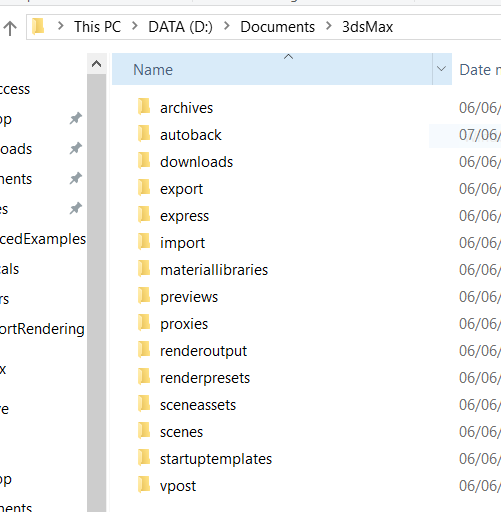
\includegraphics[width=0.5\linewidth]{img/3dsStructure.jpg}
	\caption{3D Studio Max Project Folder Structure}
	\label{fig:3dsstructure}
\end{figure}
\begin{figure}[h]
	\centering
	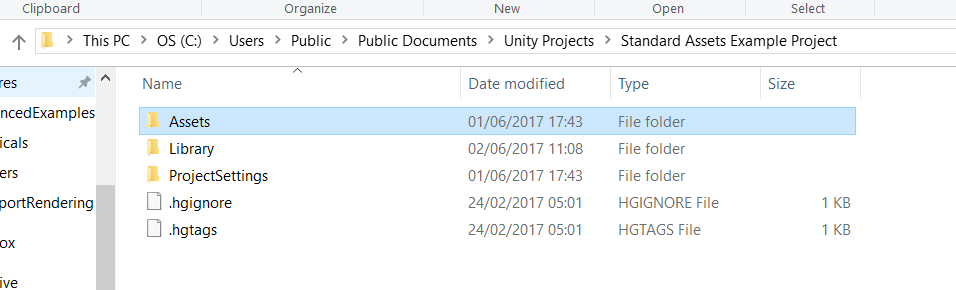
\includegraphics[width=0.9\linewidth]{img/Unity.jpg}
	\caption{Unity Game Engine File Structure}
	\label{fig:unity}
\end{figure}

All assets used during the course of the assignment are to be submitted.  All assets used and created should be placed within the appropriate folder.  To clarify, all 3ds Scene files should be placed within the 'scenes' folder; and all renders should be placed within the 'renderoutput' folder.
\\
\\
Please note that it is not appropriate to submit a single \textit{.max} file, single \textit{.jpg} file, or a single \textit{.unity} file.  

\vspace{1cm}
\textbf{Late Submission}\\
Failure to submit your assignment on or before the date and time indicated will result in a penalty of 5\% per day or part thereof.
\\
\\
Late submission penalties will not apply in cases where a valid medical certificate is provided.  In such instances an extension of time will be granted for the duration of illness stated on the medical certificate that falls after the submission date.  A copy of the medical certificate must be included with the late submission.
\\
\\
Late submission penalties may also be avoided in exceptional circumstances.  These will be dealt with on a case by case basis.  Please note that loss of pen-drives, inability to use or access the software etc. will not be considered 'exceptional circumstances'.




\end{document}